\documentclass{beamer}
\usepackage{graphicx}
\usepackage{setspace}
\usepackage{xcolor}
\usepackage{bm}
\usepackage{amssymb}
\usepackage{pifont}
\usepackage[ruled,vlined]{algorithm2e}
\usepackage{amsmath}
\usepackage{algorithmic}
\usepackage{algorithm}
\usepackage{algpseudocode}
\usepackage{caption}
\usepackage{multirow}
\usepackage{array}
\usepackage{mathrsfs}
\usepackage{tikz}

\theoremstyle{plain}
\newtheorem{window}{}

\usetheme{Madrid}
\usecolortheme{default}

% Impostazioni dell'immagine di sfondo
%\usebackgroundtemplate{\includegraphics[width=\paperwidth,height=\paperheight]{artwork.png}}

\begin{document}

\title[Explaining RF]{Explaining Random Forests with SAT}
\subtitle{Advanced Artificial Intelligence Project}
\author[Fausto, Romano]{Fausto Martina \and Romano Gabriele}
\date{\today}

\begin{frame}{Advanced Artificial Intelligence}
  \titlepage
\end{frame}

\begin{frame}{Introduction}
    \begin{block}{Goals}
        \begin{itemize}
            \item Compute the MUSes extraction as explained in On Explaining Random Forests with SAT paper by Yacine Izza and Joao Marques-Silva
            \item Implement a method to manipulate auxiliary variables introduced during the encoding process to make sure there is no collision between identifiers of the variables
            \item Implement a method to differentiate the majority voting encoding in the case with two classes and in the case with more classes
        \end{itemize}
    \end{block}
    \vfill
    \begin{center}
        \fontsize{7}{10}\selectfont
        \textbf{GITHUB REPOSITORY}\\
        \url{https://github.com/yizza91/RFxpl}
    \end{center}
\end{frame}

\begin{frame}{Introduction}
    \begin{block}{Proposed Paper}
    %\fontsize{7}{10}\selectfont
        \begin{itemize}
            \item Brief introduction to ML Classification, Decision Trees and Random Forest Classifiers
            \item Answers the question of whether finding explanations of RFs can be solved in polynomial time negatively, by proving that deciding whether a set of literals is a PI-explanation of an RF is DP-complete
            \item Proposes a propositional encoding for computing explanations of RFs, thus enabling finding PI-explanations with a SAT solver
            \item Experimental findings, derived from an extensive array of publicly accessible datasets, highlight a substantial performance improvement in the proposed SAT-based method compared to existing heuristic approaches
        \end{itemize}
    \end{block}
\end{frame}

\begin{frame}{Introduction}
    \begin{block}{Symbology}
        \begin{itemize}
            \item \(\mathcal{F}\) = \( \{ 1, ..., m \} \) is the set of features
            \item \(\mathcal{K}\) = \( \{ c_{1}, ..., c_{K} \} \) is the set of classes
            \item $\mathbf{x}$ = \( \{ x_{1}, ..., x_{m} \} \) is an arbitrary point in the feature space $\mathbb{F}$
            \item $\mathbf{v}$ = \( \{ v_{1}, ..., v_{m} \} \) is an specific point in the feature space $\mathbb{F}$
            \item A pair ($\mathbf{v}$, c) is an instance where $\mathbf{v} \in \mathbb{F}$ and c $\in \mathcal{K}$
            \item M is the number of trees of the Random Forest
            \item $\mathcal{T}_{i}$ is the \textit{i}-th tree
            \item $l_{ik}$ is the classification $c_{k}$ for the \textit{i}-th tree
            \item \(\mathcal{R}_{i}\) is the set of paths of \(\mathcal{T}_{i}\)
            \item R$_{k}$ is the $k$-th path of a set \(\mathcal{R}_{i}\)
        \end{itemize}
    \end{block}
\end{frame}
\begin{frame}{Paths}
    \begin{block}{Definition}
        For every $\mathcal{T}_{i}$ encodes the set of paths $\mathcal{R}_{i}$ of $\mathcal{T}_{i}$ as follows:
        \begin{equation*}
        \bigwedge_{R_{k} \in \mathcal{R}_{i}} \left( \left( \bigwedge_{l_{j} \in \mathcal{L}(R_{k})} l_{j} \right) \rightarrow l_{ij} \right)
        \end{equation*}
        where $l_{ij}$ is a literal associated with $\mathcal{T}_{i}$ in which the voted class is $c_{j} \in \mathcal{K}$.
    \end{block}
\end{frame}

\begin{frame}{Cardinality Network}
    \begin{block}{Definition}
        For every $\mathcal{T}_{i}$ and every path R$_{k} \in \mathcal{R}_{i}$ enforces the condition that exactly one variable $l_{ij}$ is True in $\mathcal{T}_{i}$:
         \begin{equation*}
            \left( \bigvee_{j=1}^{K} l_{ij} \right) \land \left \sum_{j=1}^{K} l_{ij} \leq 1 \right
        \end{equation*}
    \end{block}
\end{frame}

\begin{frame}{Majority Voting}
    \begin{block}{Definition}
    The prediction function in RF works by majority vote, that is each tree votes for a class and the most voted class is picked. \\
    In case of ties, for simplicity we will pick the lexicographical smallest class.
    \end{block}
\end{frame}

\begin{frame}{Majority Voting Encoding}
    \begin{block}{Standard case $\textit{K}>2$}
    The Majority Voting encoding requires the use of \texit{K}-1 cardinality constraints, each comparing the counts of $c_{j}$ with the counts of some other $c_{k}$, considering $c_{k}$ as the class predicted by the RF for the instance $\mathbf{v}$.\\

    \begin{itemize}
        \item for $i \leq k < j \leq K$, $c_{k}$ is selected over $c_{j}$ if:
        \begin{equation*}
            \sum_{i=1}^{M} l_{ik} > \sum_{i=1}^{M} l_{ij} \iff \sum_{i=1}^{M} l_{ik} + \sum_{i=1}^{M} \neg l_{ij} \geq M
        \end{equation*}
        \item for $i \leq j < k \leq K$, $c_{k}$ is selected over $c_{j}$ if:
        \begin{equation*}
            \sum_{i=1}^{M} l_{ik} > \sum_{i=1}^{M} l_{ij} \iff \sum_{i=1}^{M} l_{ik} + \sum_{i=1}^{M} \neg l_{ij} \geq M+1
        \end{equation*}
    \end{itemize}
    \end{block}
\end{frame}


\begin{frame}{Majority Voting Encoding}
    \small
    \begin{block}{Special case $\textit{K}=2$}
    The Majority Voting encoding for $\textit{K}=2$ is a special case because:
    \begin{equation*}
        \footnotesize
            \sum_{i=1}^{M} l_{ik} = \sum_{i=1}^{M} \neg l_{ij} 
    \end{equation*}
    The right hand side of the standard case becomes simpler:
    \begin{itemize}
        \item for $i \leq k < j \leq K$, $c_{k}$ is selected over $c_{j}$ if:
        \begin{equation*}
            \footnotesize
            \sum_{i=1}^{M} \neg l_{ij} \geq \frac{M+1}{2}
        \end{equation*}
        \item for $i \leq j < k \leq K$, $c_{k}$ is selected over $c_{j}$ if:
        \begin{equation*}
            \footnotesize
            \sum_{i=1}^{M} \neg l_{ij} \geq \frac{M+1}{2}
        \end{equation*}
    \end{itemize}
    \end{block}
\end{frame}

\begin{frame}{Abductive Explanations (AXps)}
    \begin{block}{Definition}
        A PI-explanation (AXp) is any minimal subset  \(\mathcal{X} \subseteq \mathcal{F} \) such that:
        \begin{equation*}
            \forall (\mathbf{x} \in \mathbb{F}), \, \left[ \bigwedge_{i \in \mathcal{X}} (x_i = v_i) \right] \rightarrow (\tau(\mathbf{x}) = c)
        \end{equation*}
    \end{block}
    \begin{block}{Soft and Hard Clauses \(\langle \mathcal{H},\mathcal{S} \rangle\)}
        \begin{itemize}
            \item Soft Clause: clause that can be dropped, thus allowing it's variables to take any value
            \item Hard Clause: constraint clause that must be true for the satisfiability of the formula
        \end{itemize}
    \end{block}
\end{frame}

\begin{frame}{Abductive Explanations (AXps)}
    \footnotesize
    \begin{block}{Computing AXps}
        The set of features $\mathcal{X}$ is an AXp if the following formula is unsatisfiable:
        \begin{equation*}
            \left[ \bigwedge_{i \in \mathcal{X}} (x_i = v_i) \right] \land Enc(\tau(\mathbf{x}) \neq c)
        \end{equation*}
        This results in searching for a minimal subset $\mathcal{E} \subseteq \mathcal{S}$ such that
        \begin{equation*}
            \left[ \bigwedge_{(x_i = v_i) \in \mathcal{E}} (x_i = v_i) \right] \land Enc(\tau(\mathbf{x}) \neq c)
        \end{equation*} 
        is unsatisfiable.
        \vspace{2pt}
    \end{block}
    \begin{block}{Goal}
        Find, gradually making the variables free, the minimum feature set $\mathcal{E} \subseteq \mathcal{S}$ while still keeping the pair $\langle \mathcal{H},\mathcal{S} \rangle$ unsatisfiable.
    \end{block}
\end{frame}

\begin{frame}{Heart Disease Example - Context}
    \footnotesize
    \begin{block}{RF Running example}
        \begin{center}
        \begin{tabular}{|>{\centering \arraybackslash}p{2cm}||>{\centering \arraybackslash}p{5cm}|}
            \hline
            Paper Variable & Description\\
            \hline
            $l_{i2}$ & i-th Decision Tree answered “Yes” \\
            $l_{i1}$ & i-th Decision Tree answered “No”\\
            $x_{1}$ & “Blocked Arteries” \\
            $x_{2}$ & “Good-Blood Circulation”\\
            $x_{3}$ & “Chest-Pain”\\
            $w$ & “Weight \(>\) 75”\\
            \hline
        \end{tabular}
        \begin{center}
            \begin{minipage}{0.175\linewidth}
                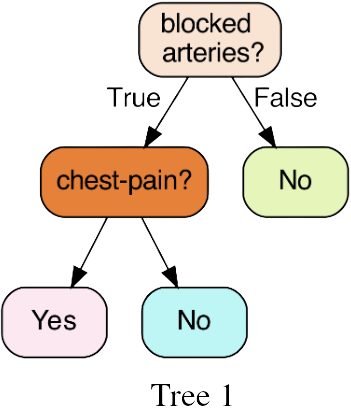
\includegraphics[width=\textwidth]{resources/RF_1.png}
            \end{minipage}
            \hspace{8pt}
            \begin{minipage}{0.175\linewidth}
                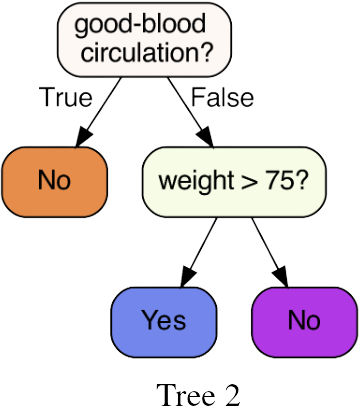
\includegraphics[width=\textwidth]{resources/RF_2.png}
            \end{minipage}
            \hspace{8pt}
            \begin{minipage}{0.265\linewidth}
                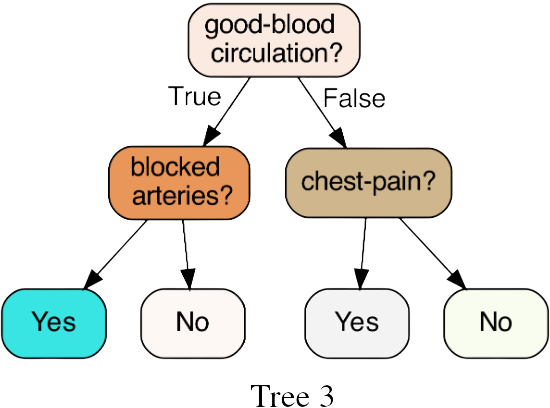
\includegraphics[width=\textwidth]{resources/RF_3.png}
            \end{minipage}
        \end{center}
        The instance $\textbf{v} = ((1,0,1,70), Yes)$ results in the soft clauses: $\{x_{1}\},\{ \lnot x_{2}\},\{x_{3}\},\{\lnot w\}$
        \vspace{2pt}
        \end{center}
    \end{block}
\end{frame}



\begin{frame}{Heart Disease Example - Step 0}
    \centering
    \fontsize{8pt}{1pt}\selectfont 
    \linespread{0.6}
    \begin{minipage}[t]{0.22\textwidth}
        \begin{block}{\centering \fontsize{8.5pt}{0pt}\selectfont \textbf{Paths}}
            \linespread{0.1}
            \[\{l_{12} , \lnot x_{1} , \lnot x_{3}\},\]
            \linespread{0.2}
            
            \[\{l_{11} , \lnot x_{1} , x_{3}\},\]
            
            \[\{l_{11} , x_{1}\},\]
            
            \[\{l_{21} , \lnot x_{2}\},\]
            
            \[\{l_{22} , x_{2}  , \lnot w\},\]
            
            \[\{l_{21} , x_{2}  , w\},\]
            
            \[\{l_{32} , \lnot x_{2} ,\lnot x_{1}\},\]
            
            \[\{l_{31} , \lnot x_{2} , x_{1}\},\]
            
            \[\{l_{32} , x_{2} , \lnot x_{3}\},\]
            
            \[\{l_{31} , x_{2} , x_{3}\},\]
            \vspace{2pt}
        \end{block}
    \end{minipage}
    \hspace{0.05\textwidth}
    \begin{minipage}[t]{0.19\textwidth}
        \begin{block}{\centering \fontsize{8.5pt}{2pt}\selectfont \textbf{Cardinality Network}}
            \linespread{0.3}
            \[\{l_{11} , l_{12}\},\]
            
            \[\{\lnot l_{11} , \lnot l_{12}\},\]
            
            \[\{l_{21} , l_{22}\},\]
            
            \[\{\lnot l_{21} , \lnot l_{22}\},\]
            
            \[\{l_{31} , l_{32}\},\]
            
            \[\{\lnot l_{31} , \lnot l_{32}\},\]
            \vspace{2pt}
        \end{block}
    \end{minipage}
    \hspace{0.05\textwidth}
    \begin{minipage}[t]{0.18\textwidth}
        \begin{block}{\centering \fontsize{8.5pt}{2pt}\selectfont \textbf{Majority \\ Voting}}
            \linespread{0.1}
            \[\{\lnot l_{12} , aux_{1}\},\]
            \linespread{0.3}
            
            \[\{\lnot aux_{1}, aux_{2}\},\]
            
            \[\{\lnot l_{22} , \lnot aux_{1}\},\]
            
            \[\{\lnot l_{22} , aux_{2}\},\]
            
            \[\{\lnot l_{32} , \lnot aux_{2}\},\]
            \vspace{2pt}
        \end{block}
    \end{minipage}
    \hspace{0.05\textwidth}
    \begin{minipage}[t]{0.12\textwidth}
        \begin{block}{\centering \fontsize{8.5pt}{2pt}\selectfont \textbf{Soft Clauses}}
            \linespread{0.3}
            \[\{x_{1}\},\]
            
            \[\{\lnot x_{2}\},\]
            
            \[\{x_{3}\},\]
            
            \[\{\lnot w\}\]
        \end{block}
        \vspace{10pt}
        \begin{block}{\centering \fontsize{8.5pt}{1pt}\selectfont \textbf{Implicit Clauses}}
            \vspace{5pt}
        \end{block}
    \end{minipage}
\end{frame}


\begin{frame}{Heart Disease Example - Step 1}
    \centering
    \fontsize{8pt}{1pt}\selectfont 
    \linespread{0.6}
    \begin{minipage}[t]{0.22\textwidth}
        \begin{block}{\centering \fontsize{8.5pt}{0pt}\selectfont \textbf{Paths}}
            \linespread{0.1}
            \only<1>{\[\{l_{12} , \lnot x_{1} ,\lnot x_{3}\},\]}
            \only<2->{\[\colorbox[HTML]{C8FAC8}{\(\{l_{12} , \textcolor[HTML]{008000}{\bm{\lnot x_{1}}} , \textcolor{red}{\bm{\lnot x_{3}}}\},\)}\]}
            \only<1>{\linespread{0.3}}
            \only<2>{\linespread{0.1}}
            \only<3->{\linespread{0}}
            
            \only<1>{\[\{l_{11} ,\lnot x_{1} , x_{3}\},\]}
            \only<2->{\[\colorbox[HTML]{C8FAC8}{\(\{l_{11} , \textcolor[HTML]{008000}{\bm{\lnot x_{1}}} , \textcolor[HTML]{008000}{\bm{x_{3}}}\},\)}\]}
            
            \only<1>{\[\{l_{11} , x_{1}\},\]}
            \only<2>{\[\{l_{11} , \textcolor{red}{\bm{x_{1}}}\},\]}
            \only<3->{\[\colorbox[HTML]{C8FAC8}{\(\{\textcolor[HTML]{008000}{\bm{l_{11}}} , \textcolor{red}{\bm{x_{1}}}\},\)}\]}
            
            \only<1>{\[\{l_{21} ,\lnot x_{2}\},\]}
            \only<2->{\[\colorbox[HTML]{C8FAC8}{\(\{l_{21} , \textcolor[HTML]{008000}{\bm{\lnot x_{2}}}\},\)}\]}
            
            \only<1>{\[\{l_{22} ,x_{2} ,\lnot w\},\]}
            \only<2->{\[\colorbox[HTML]{C8FAC8}{\(\{l_{22} , \textcolor{red}{\bm{x_{2}}}  , \textcolor[HTML]{008000}{\bm{\lnot w}}\},\)}\]}
            
            \only<1>{\[\{l_{21} , x_{2}  , w\},\]}
            \only<2>{\[\{l_{21} , \textcolor{red}{\bm{x_{2}}}  , \textcolor{red}{\bm{w}}\},\]}
            \only<3->{\[\colorbox[HTML]{C8FAC8}{\(\{\textcolor[HTML]{008000}{\bm{l_{21}}} , \textcolor{red}{\bm{x_{2}}}  , \textcolor{red}{\bm{w}}\},\)}\]}
            
            \only<1>{\[\{l_{32} ,\lont x_{2} ,\lnot x_{1}\},\]}
            \only<2->{\[\colorbox[HTML]{C8FAC8}{\(\{l_{32} , \textcolor[HTML]{008000}{\bm{\lnot x_{2}}} , \textcolor[HTML]{008000}{\bm{\lnot x_{1}}}\},\)}\]}
            
            \only<1>{\[\{l_{31} ,\lnot x_{2} , x_{1}\},\]}
            \only<2->{\[\colorbox[HTML]{C8FAC8}{\(\{l_{31} , \textcolor[HTML]{008000}{\bm{\lnot x_{2}}} , \textcolor{red}{\bm{x_{1}}}\},\)}\]}
            
            \only<1>{\[\{l_{32} , x_{2} , \lnot x_{3}\},\]}
            \only<2>{\[\{l_{32} , \textcolor{red}{\bm{x_{2}}} , \textcolor{red}{\bm{\lnot x_{3}}}\},\]}
            \only<3->{\[\colorbox[HTML]{C8FAC8}{\(\{\textcolor[HTML]{008000}{\bm{l_{32}}} , \textcolor{red}{\bm{x_{2}}} , \textcolor{red}{\bm{\lnot x_{3}}}\},\)}\]}
            
            \only<1>{\[\{l_{31} ,x_{2} ,x_{3}\},\]}
            \only<2->{\[\colorbox[HTML]{C8FAC8}{\(\{l_{31} , \textcolor{red}{\bm{x_{2}}} , \textcolor[HTML]{008000}{\bm{x_{3}}}\},\)}\]}
            \only<1>{\vspace{2pt}}
        \end{block}
    \end{minipage}
    \hspace{0.05\textwidth}
    \begin{minipage}[t]{0.19\textwidth}
        \begin{block}{\centering \fontsize{8.5pt}{2pt}\selectfont \textbf{Cardinality Network}}
            \only<1-2>{\linespread{0.5}}
            \only<3>{\linespread{0.3}}
            \only<4->{\linespread{0.15}}
            \only<1-2>{\[\{l_{11} , l_{12}\},\]}
            \only<3->{\[\colorbox[HTML]{C8FAC8}{\(\{\textcolor[HTML]{008000}{\bm{l_{11}}} , l_{12}\},\)}\]}
            
            \only<1-2>{\[\{\lnot l_{11} , \lnot l_{12}\},\]}
            \only<3>{\[\{\textcolor{red}{\bm{\lnot l_{11}}} , \lnot l_{12}\},\]}
            \only<4->{\[\colorbox[HTML]{C8FAC8}{\(\{\textcolor{red}{\bm{\lnot l_{11}}} , \textcolor[HTML]{008000}{\bm{\lnot l_{12}}}\},\)}\]}
            
            \only<1-2>{\[\{l_{21} , l_{22}\},\]}
            \only<3->{\[\colorbox[HTML]{C8FAC8}{\(\{\textcolor[HTML]{008000}{\bm{l_{21}}} , l_{22}\},\)}\]}
            
            \only<1-2>{\[\{\lnot l_{21}, \lnot l_{22}\},\]}
            \only<3>{\[\{\textcolor{red}{\bm{\lnot l_{21}}} , \lnot l_{22}\},\]}
            \only<4->{\[\colorbox[HTML]{C8FAC8}{\(\{\textcolor{red}{\bm{\lnot l_{21}}} , \textcolor[HTML]{008000}{\bm{\lnot l_{22}}}\},\)}\]}
            
            \only<1-2>{\[\{l_{31} , l_{32}\},\]}
            \only<3->{\[\colorbox[HTML]{C8FAC8}{\(\{l_{31} , \textcolor[HTML]{008000}{\bm{l_{32}}}\},\)}\]}
            
            \only<1-2>{\[\{\lnot l_{31} , \lnot l_{32}\},\]}
            \only<3>{\[\{\lnot l_{31} , \textcolor{red}{\bm{\lnot l_{32}}}\},\]}
            \only<4->{\[\colorbox[HTML]{C8FAC8}{\(\{\textcolor[HTML]{008000}{\bm{\lnot l_{31}}} , \textcolor{red}{\bm{\lnot l_{32}}}\},\)}\]}
            \vspace{2pt}
        \end{block}
    \end{minipage}
    \hspace{0.05\textwidth}
    \begin{minipage}[t]{0.18\textwidth}
        \begin{block}{\centering \fontsize{8.5pt}{2pt}\selectfont \textbf{Majority \\ Voting}}
            \linespread{0.1}
            \only<1-3>{\[\{\lnot l_{12} , aux_{1}\},\]}
            \only<4->{\[\colorbox[HTML]{C8FAC8}{\(\{\textcolor[HTML]{008000}{\bm{\lnot l_{12}}} , aux_{1}\},\)}\]}
            \only<1-3>{\linespread{0.5}}
            \only<4>{\linespread{0.2}}
            \only<5>{\linespread{0.1}}
            
            \only<1-3>{\[\{\lnot aux_{1}, aux_{2}\},\]}
            \only<4>{\[\{\lnot aux_{1}, \textcolor{red}{\bm{aux_{2}}}\},\]}
            \only<5->{\[\colorbox[HTML]{C8FAC8}{\(\{\textcolor[HTML]{008000}{\bm{\lnot aux_{1}}}, \textcolor{red}{\bm{aux_{2}}}\},\)}\]}
            
            \only<1-3>{\[\{\lnot l_{22} , \lnot aux_{1}\},\]}
            \only<4->{\[\colorbox[HTML]{C8FAC8}{\(\{\textcolor[HTML]{008000}{\bm{\lnot l_{22}}} , \lnot aux_{1}\},\)}\]}
            
            \only<1-3>{\[\{\lnot l_{22} , aux_{2}\},\]}
            \only<4->{\[\colorbox[HTML]{C8FAC8}{\(\{\textcolor[HTML]{008000}{\bm{\lnot l_{22}}} , \textcolor{red}{\bm{aux_{2}}}\},\)}\]}
            
            \only<1-2>{\[\{\lnot l_{32} , \lnot aux_{2}\},\]}
            \only<3>{\[\{\textcolor{red}{\bm{\lnot l_{32}}} , \lnot aux_{2}\},\]}
            \only<4->{\[\colorbox[HTML]{C8FAC8}{\(\{\textcolor{red}{\bm{\lnot l_{32}}} , \textcolor[HTML]{008000}{\bm{\lnot aux_{2}}}\},\)}\]}
            \vspace{1pt}
        \end{block}
    \end{minipage}
    \hspace{0.05\textwidth}
    \begin{minipage}[t]{0.12\textwidth}
        \begin{block}{\centering \fontsize{8.5pt}{2pt}\selectfont \textbf{Soft Clauses}}
            \only<1>{\linespread{0.2}}
            \only<2->{\linespread{0}}
            \only<1>{\vspace{1}\[\{\lnot x_{2}\},\]\vspace{1}}
            \only<2->{\begin{align} \colorbox[HTML]{C8FAC8}{\(\textcolor[HTML]{008000}{\textbf{\[\{\bm{\lnot x_{2}}\},\]}}\)} \end{align}}
            
            \only<1>{\linespread{0.1}}
            \only<2->{\linespread{0}}
            \only<1>{\vspace{1}\[\{x_{3}\},\]\vspace{1}}
            \only<2->{\begin{align} \colorbox[HTML]{C8FAC8}{\(\textcolor[HTML]{008000}{\textbf{\[\{\bm{x_{3}}\},\]}}\)} \end{align}}
            
            \only<1>{\vspace{1}\[\{\lnot w\},\]\vspace{1}}
            \only<2->{\begin{align} \colorbox[HTML]{C8FAC8}{\(\textbf{\color[HTML]{008000}{\[\{\bm{\lnot w}\},\]}}\)} \end{align}}
            \vspace{1pt}
        \end{block}
        \vspace{25pt}
        \begin{block}{\centering \fontsize{8.5pt}{1pt}\selectfont \textbf{Implicit Clauses}}
            \linespread{0.1}
            \only<1>{\[\{\lnot x_{1}\}\]}
            \only<2->{\[\begin{align} \colorbox[HTML]{C8FAC8}{\(\textcolor[HTML]{008000}{\{\bm{\lnot x_{1}}\}}\)}\] \end{align}}
        \end{block}
    \end{minipage}
    \vspace{2pt}
    \\
    \only<1-4>{\textcolor{white}{The formula is \colorbox[HTML]{FFFFFF}{SATISFIABLE}: $(\lnot x_{2} \},\{ x_{3} \},\{ \lnot w)$ is not an AXp candidate\\}}
    \only<5>{The formula is \colorbox[HTML]{C8FAC8}{SATISFIABLE}: $\{\lnot x_{2} \},\{ x_{3} \},\{\lnot w\}$ is not an AXp candidate\\}
\end{frame}



\begin{frame}{Heart Disease Example - Step 2}
    \centering
    \fontsize{8pt}{1pt}\selectfont 
    \linespread{0.6}
    \begin{minipage}[t]{0.22\textwidth}
        \begin{block}{\centering \fontsize{8.5pt}{0pt}\selectfont \textbf{Paths}}
            \only<1-2>{\linespread{0.1}}
            \only<3->{\linespread{0}}
            \only<1>{\[\{l_{12} , \lnot x_{1} ,\lnot x_{3}\},\]}
            \only<2>{\[\{l_{12} , \textcolor{red}{\bm{\lnot x_{1}}} , \textcolor{red}{\bm{\lnot x_{3}}}\},\]}
            \only<3->{\[\colorbox[HTML]{C8FAC8}{\(\{\textcolor[HTML]{008000}{\bm{l_{12}}} , \textcolor{red}{\bm{\lnot x_{1}}} , \textcolor{red}{\bm{\lnot x_{3}}}\},\)}\]}
            \only<1>{\linespread{0.3}}
            \only<2>{\linespread{0.1}}
            \only<3->{\linespread{0}}
            
            \only<1>{\[\{l_{11} ,\lnot x_{1} , x_{3}\},\]}
            \only<2->{\[\colorbox[HTML]{C8FAC8}{\(\{l_{11} , \textcolor{red}{\bm{\lnot x_{1}}} , \textcolor[HTML]{008000}{\textbf{\[\bm{x_{3}}\]}}\},\)}\]}
            
            \only<1>{\[\{l_{11} , x_{1}\},\]}
            \only<2->{\[\colorbox[HTML]{C8FAC8}{\(\{l_{11} , \textcolor[HTML]{008000}{\textbf{\[\bm{x_{1}}\]}}\},\)}\]}
            
            \only<1>{\[\{l_{21} ,\lnot x_{2}\},\]}
            \only<2>{\[\{l_{21} , \textcolor{red}{\bm{\lnot x_{2}}}\},\]}
            \only<3->{\[\colorbox[HTML]{C8FAC8}{\(\{\textcolor[HTML]{008000}{\bm{l_{21}}} , \textcolor{red}{\bm{\lnot x_{2}}}\},\)}\]}
            
            \only<1>{\[\{l_{22} , x_{2} ,\lnot w\},\]}
            \only<2->{\[\colorbox[HTML]{C8FAC8}{\(\{l_{22} , \textcolor[HTML]{008000}{\bm{x_{2}}}  , \textbf{\color[HTML]{008000}{\[\bm{\lnot w}\]}}\},\)}\]}
            
            \only<1>{\[\{l_{21} , x_{2} , w\},\]}
            \only<2->{\[\colorbox[HTML]{C8FAC8}{\(\{l_{21} , \textcolor[HTML]{008000}{\bm{x_{2}}}  , \textcolor{red}{\bm{w}}\},\)}\]}
            
            \only<1>{\[\{l_{32} , \lnot x_{2} , \lnot x_{1}\},\]}
            \only<2>{\[\{l_{32} , \textcolor{red}{\bm{\lnot x_{2}}} , \textcolor{red}{\bm{\lnot x_{1}}}\},\]}
            \only<3->{\[\colorbox[HTML]{C8FAC8}{\(\{\textcolor[HTML]{008000}{\bm{l_{32}}} , \textcolor{red}{\bm{\lnot x_{2}}} , \textcolor{red}{\bm{\lnot x_{1}}}\},\)}\]}
            
            \only<1>{\[\{l_{31} ,\lnot x_{2} , x_{1}\},\]}
            \only<2->{\[\colorbox[HTML]{C8FAC8}{\(\{l_{31} , \textcolor{red}{\bm{\lnot x_{2}}} , \textcolor[HTML]{008000}{\textbf{\[\bm{x_{1}}\]}}\},\)}\]}
            
            \only<1>{\[\{l_{32} ,x_{2} ,\lnot x_{3}\},\]}
            \only<2->{\[\colorbox[HTML]{C8FAC8}{\(\{l_{32} , \textcolor[HTML]{008000}{\bm{x_{2}}} , \textcolor{red}{\bm{\lnot x_{3}}}\},\)}\]}
            
            \only<1>{\[\{l_{31} ,x_{2} ,x_{3}\},\]}
            \only<2->{\[\colorbox[HTML]{C8FAC8}{\(\{l_{31} , \textcolor[HTML]{008000}{\bm{x_{2}}} , \textcolor[HTML]{008000}{\textbf{\[\bm{x_{3}}\]}}\},\)}\]}
            \only<1>{\vspace{2pt}}
        \end{block}
    \end{minipage}
    \hspace{0.05\textwidth}
    \begin{minipage}[t]{0.19\textwidth}
        \begin{block}{\centering \fontsize{8.5pt}{2pt}\selectfont \textbf{Cardinality Network}}
            \only<1-2>{\linespread{0.1}}
            \only<3->{\linespread{0}}
            \only<1-2>{\[\{l_{11} , l_{12}\},\]}
            \only<3->{\[\colorbox[HTML]{C8FAC8}{\(\{l_{11} , \textcolor[HTML]{008000}{\bm{l_{12}}}\},\)}\]}
            \only<1-2>{\linespread{0.4}}
            \only<3>{\linespread{0.2}}
            \only<4->{\linespread{0}}
            
            \only<1-2>{\[\{\lnot l_{11} , \lnot l_{12}\},\]}
            \only<3>{\vspace{1}\[\{\lnot l_{11} , \textcolor{red}{\bm{\lnot l_{12}}}\},\]}
            \only<4->{\[\colorbox[HTML]{C8FAC8}{\(\{\textcolor[HTML]{008000}{\bm{\lnot l_{11}}} , \textcolor{red}{\bm{\lnot l_{12}}}\},\)}\]}
            
            \only<1-2>{\[\{l_{21} , l_{22}\},\]}
            \only<3->{\[\colorbox[HTML]{C8FAC8}{\(\{\textcolor[HTML]{008000}{\bm{l_{21}}} , l_{22}\},\)}\]}
            
            \only<1-2>{\[\{\lnot l_{21} , \lnot l_{22}\},\]}
            \only<3>{\[\{\textcolor{red}{\bm{\lnot l_{21}}} , \lnot l_{22}\},\]}
            \only<4->{\[\colorbox[HTML]{C8FAC8}{\(\{\textcolor{red}{\bm{\lnot l_{21}}} , \textcolor[HTML]{008000}{\bm{\lnot l_{22}}}\},\)}\]}
            
            \only<1-2>{\[\{l_{31} , l_{32}\},\]}
            \only<3->{\[\colorbox[HTML]{C8FAC8}{\(\{l_{31} , \textcolor[HTML]{008000}{\bm{l_{32}}}\},\)}\]}
            
            \only<1-2>{\[\{\lnot l_{31} , \lnot l_{32}\},\]}
            \only<3>{\[\{\lnot l_{31} , \textcolor{red}{\bm{\lnot l_{32}}}\},\]}
            \only<4->{\[\colorbox[HTML]{C8FAC8}{\(\{\textcolor[HTML]{008000}{\bm{\lnot l_{31}}} , \textcolor{red}{\bm{\lnot l_{32}}}\},\)}\]}
        \end{block}
    \end{minipage}
    \hspace{0.05\textwidth}
    \begin{minipage}[t]{0.18\textwidth}
        \begin{block}{\centering \fontsize{8.5pt}{2pt}\selectfont \textbf{Majority \\ Voting}}
            \only<1-3>{\linespread{0.35}}
            \only<4>{\linespread{0}}
            \only<1-2>{\[\{\lnot l_{12} , aux_{1}\},\]}
            \only<3>{\[\{\textcolor{red}{\bm{\lnot l_{12}}} , aux_{1}\},\]}
            \only<4->{\[\colorbox[HTML]{C8FAC8}{\(\{\textcolor{red}{\bm{\lnot l_{12}}} , \textcolor[HTML]{008000}{\bm{aux_{1}}}\},\)}\]}
            \only<1-3>{\linespread{0.5}}
            \only<4->{\linespread{0.1}}
            
            \only<1-3>{\[\{\lnot aux_{1} , aux_{2}\},\]}
            \only<4->{\[\colorbox[HTML]{FAC8C8}{\(\{\textcolor{red}{\bm{\lnot aux_{1}}} , \textcolor{red}{\bm{aux_{2}}}\},\)}\]}
            
            \only<1-3>{\[\{\lnot l_{22} , \lnot aux_{1}\},\]}
            \only<4->{\[\colorbox[HTML]{C8FAC8}{\(\{\textcolor[HTML]{008000}{\bm{\lnot l_{22}}} , \textcolor{red}{\bm{\lnot aux_{1}}}\},\)}\]}
            
            \only<1-3>{\[\{\lnot l_{22} , aux_{2}\},\]}
            \only<4->{\[\colorbox[HTML]{C8FAC8}{\(\{\textcolor[HTML]{008000}{\bm{\lnot l_{22}}} , \textcolor{red}{\bm{aux_{2}}}\},\)}\]}
            
            \only<1-2>{\[\{\lnot l_{32} , \lnot aux_{2}\},\]}
            \only<3>{\[\{\textcolor{red}{\bm{\lnot l_{32}}} , \lnot aux_{2}\},\]}
            \only<4->{\[\colorbox[HTML]{C8FAC8}{\(\{\textcolor{red}{\bm{\lnot l_{32}}} , \textcolor[HTML]{008000}{\bm{\lnot aux_{2}}}\},\)}\]}
            \only<4>{\vspace{0.4}}
        \end{block}
    \end{minipage}
    \hspace{0.05\textwidth}
    \begin{minipage}[t]{0.12\textwidth}
        \begin{block}{\centering \fontsize{8.5pt}{2pt}\selectfont \textbf{Soft Clauses}}
            \only<1>{\linespread{0.2}}
            \only<2->{\linespread{0}}
            \only<1>{\vspace{1}\[\{x_{1}\},\]\vspace{1}}
            \only<2->{\begin{align} \colorbox[HTML]{C8FAC8}{\(\textcolor[HTML]{008000}{\textbf{\[\{\bm{x_{1}}\},\]}}\)} \end{align}}
            \only<1>{\linespread{0.5}}
            \only<2->{\linespread{0}}
            
            \only<1>{\[\{x_{3}\},\]}
            \only<2->{\begin{align} \colorbox[HTML]{C8FAC8}{\(\textcolor[HTML]{008000}{\textbf{\[\{\bm{x_{3}}\},\]}}\)} \end{align}}
            
            \only<1>{\[\{\lnot w\},\]}
            \only<2->{\begin{align} \colorbox[HTML]{C8FAC8}{\(\textbf{\color[HTML]{008000}{\[\{\bm{\lnot w}\},\]}}\)} \end{align}}
        \end{block}
        \only<1-> {
            \vspace{10pt}
            \begin{block}{\centering \fontsize{8.5pt}{2pt}\selectfont \textbf{Implicit Clauses}}
                \linespread{0}
                \only<1>{\vspace{1} \[\{x_{2}\}\] \vspace{1}}
                \only<2->{\begin{align*} \colorbox[HTML]{C8FAC8}{\(\textcolor[HTML]{008000}{\{\bm{x_{2}}\}}\)} \end{align*}}
            \end{block}
        }
    \end{minipage}
    \vspace{2pt}
    \\
    \only<1-3>{\textcolor{white}{The formula is \colorbox[HTML]{FFFFFF}{UNSATISFIABLE}: $(x_{1} \},\{ x_{3} \},\{ \lnot w)$ is a valid AXp candidate. we start dropping variables...}}
    \only<4>{The formula is \colorbox[HTML]{FAC8C8}{UNSATISFIABLE}: $\{x_{1} \},\{x_{3} \},\{\lnot  w\}$ is a valid AXp candidate.}
\end{frame}


\begin{frame}{Heart Disease Example - Step 3}
    \centering
    \fontsize{8pt}{1pt}\selectfont 
    \linespread{0.6}
    \begin{minipage}[t]{0.22\textwidth}
        \begin{block}{\centering \fontsize{8.5pt}{0pt}\selectfont \textbf{Paths}}
            \only<1>{\linespread{0.2}}
            \only<2->{\linespread{0}}
            \only<1>{\[\{l_{12} , \lnot x_{1} ,\lnot x_{3}\},\]}
            \only<2->{\[\colorbox[HTML]{C8FAC8}{\(\{l_{12} , \textcolor[HTML]{008000}{\bm{\lnot x_{1}}} , \textcolor{red}{\textbf{\[\bm{\lnot x_{3}}\]}}\)}\]}
            \only<1>{\linespread{0.3}}
            \only<2->{\linespread{0}}
            
            \only<1>{\[\{l_{11} ,\lnot x_{1} , x_{3}\},\]}
            \only<2->{\[\colorbox[HTML]{C8FAC8}{\(\{l_{11} , \textcolor[HTML]{008000}{\bm{\lnot x_{1}}} , \textcolor[HTML]{008000}{\textbf{\[\bm{ x_{3}}\]}}\},\)}\]}
            
            \only<1>{\[\{l_{11} , x_{1}\},\]}
            \only<2->{\[\colorbox[HTML]{C8FAC8}{\(\{\textcolor[HTML]{008000}{\bm{l_{11}}} , \textcolor{red}{\bm{x_{1}}}\},\)}\]}
            
            \only<1>{\[\{l_{21} ,\lnot x_{2}\},\]}
            \only<2->{\[\colorbox[HTML]{C8FAC8}{\(\{\textcolor[HTML]{008000}{\bm{l_{21}}} , \textcolor{red}{\bm{\lnot x_{2}}}\},\)}\]}
            
            \only<1>{\[\{l_{22} , x_{2},\lnot w\},\]}
            \only<2->{\[\colorbox[HTML]{C8FAC8}{\(\{l_{22} , \textcolor[HTML]{008000}{\bm{x_{2}}}  , \textcolor[HTML]{008000}{\bm{\lnot w}}\},\)}\]}
            
            \only<1>{\[\{l_{21} ,x_{2}, w\},\]}
            \only<2->{\[\colorbox[HTML]{C8FAC8}{\(\{l_{21} , \textcolor[HTML]{008000}{\bm{x_{2}}}  , \textcolor{red}{\bm{w}}\},\)}\]}
            
            \only<1>{\[\{l_{32} , \lnot x_{2}, \lnot x_{1}\},\]}
            \only<2->{\[\colorbox[HTML]{C8FAC8}{\(\{l_{32} , \textcolor{red}{\bm{\lnot x_{2}}} , \textcolor[HTML]{008000}{\bm{\lnot x_{1}}}\},\)}\]}
            
            \only<1>{\[\{l_{31} ,\lnot x_{2} ,x_{1}\},\]}
            \only<2->{\[\colorbox[HTML]{C8FAC8}{\(\{\textcolor[HTML]{008000}{\bm{l_{31}}} , \textcolor{red}{\bm{\lnot x_{2}}} , \textcolor{red}{\bm{x_{1}}}\},\)}\]}
            
            \only<1>{\[\{l_{32} , x_{2} , \lnot x_{3}\},\]}
            \only<2->{\[\colorbox[HTML]{C8FAC8}{\(\{l_{32} , \textcolor[HTML]{008000}{\bm{x_{2}}} , \textcolor{red}{\bm{\lnot x_{3}}}\},\)}\]}
            
            \only<1>{\[\{l_{31} ,x_{2} , x_{3}\},\]}
            \only<2->{\[\colorbox[HTML]{C8FAC8}{\(\{l_{31} , \textcolor[HTML]{008000}{\bm{x_{2}}} , \textcolor[HTML]{008000}{\bm{x_{3}}}\},\)}\]}
        \end{block}
    \end{minipage}
    \hspace{0.05\textwidth}
    \begin{minipage}[t]{0.19\textwidth}
        \begin{block}{\centering \fontsize{8.5pt}{2pt}\selectfont \textbf{Cardinality Network}}
            \only<1>{\linespread{0.3}}
            \only<2->{\linespread{0}}
            \only<1>{\[\{l_{11} , l_{12}\},\]}
            \only<2->{\[\colorbox[HTML]{C8FAC8}{\(\{\textcolor[HTML]{008000}{\bm{l_{11}}} , l_{12}\},\)}\]}
            \only<1>{\linespread{0.3}}
            \only<2->{\linespread{0}}
            
            \only<1>{\[\{\lnot l_{11} , \lnot l_{12}\},\]}
            \only<2->{\[\colorbox[HTML]{C8FAC8}{\(\{\textcolor{red}{\bm{\lnot l_{11}}} , \textcolor[HTML]{008000}{\bm{\lnot l_{12}}}\},\)}\]}
            
            \only<1>{\[\{l_{21} , l_{22}\},\]}
            \only<2->{\[\colorbox[HTML]{C8FAC8}{\(\{\textcolor[HTML]{008000}{\bm{l_{21}}} , l_{22}\},\)}\]}
            
            \only<1>{\[\{\lnot l_{21} , \lnot l_{22}\},\]}
            \only<2->{\[\colorbox[HTML]{C8FAC8}{\(\{\textcolor{red}{\bm{\lnot l_{21}}} , \textcolor[HTML]{008000}{\bm{\lnot l_{22}}}\},\)}\]}
            
            \only<1>{\[\{l_{31} , l_{32}\},\]}
            \only<2->{\[\colorbox[HTML]{C8FAC8}{\(\{\textcolor[HTML]{008000}{\bm{l_{31}}} , l_{32}\},\)}\]}
            
            \only<1>{\[\{\lnot l_{31} , \lnot l_{32}\},\]}
            \only<2->{\[\colorbox[HTML]{C8FAC8}{\(\{\textcolor{red}{\bm{\lnot l_{31}}} , \textcolor[HTML]{008000}{\bm{\lnot l_{32}}}\},\)}\]}
        \end{block}
    \end{minipage}
    \hspace{0.05\textwidth}
    \begin{minipage}[t]{0.18\textwidth}
        \begin{block}{\centering \fontsize{8.5pt}{2pt}\selectfont \textbf{Majority \\ Voting}}
            \only<1>{\linespread{0.1}}
            \only<2->{\linespread{0}}
            \only<1>{\[\{\lnot l_{12} , aux_{1}\},\]}
            \only<2->{\[\colorbox[HTML]{C8FAC8}{\(\{\textcolor[HTML]{008000}{\bm{\lnot l_{12}}} , aux_{1}\},\)}\]}
            \only<1>{\linespread{0.3}}
            \only<2->{\linespread{0}}
            
            \only<1>{\[\{\lnot aux_{1} , aux_{2}\},\]}
            \only<2->{\[\colorbox[HTML]{C8FAC8}{\(\{\textcolor[HTML]{008000}{\bm{\lnot aux_{1}}} , aux_{2}\},\)}\]}
            
            \only<1>{\[\{\lnot l_{22} , \lnot aux_{1}\},\]}
            \only<2->{\[\colorbox[HTML]{C8FAC8}{\(\{\textcolor[HTML]{008000}{\bm{\lnot l_{22}}} , \lnot aux_{1}\},\)}\]}
            
            \only<1>{\[\{\lnot l_{22} , aux_{2}\},\]}
            \only<2->{\[\colorbox[HTML]{C8FAC8}{\(\{\textcolor[HTML]{008000}{\bm{\lnot l_{22}}} , aux_{2}\},\)}\]}
            
            \only<1>{\[\{\lnot l_{32} , \lnot aux_{2}\},\]}
            \only<2->{\[\colorbox[HTML]{C8FAC8}{\(\{\textcolor[HTML]{008000}{\bm{\lnot l_{32}}} , \lnot aux_{2}\},\)}\]}
        \end{block}
    \end{minipage}
    \hspace{0.05\textwidth}
    \begin{minipage}[t]{0.12\textwidth}
        \begin{block}{\centering \fontsize{8.5pt}{2pt}\selectfont \textbf{Soft Clauses}}
            \only<1>{\linespread{0.2}}
            \only<2->{\linespread{0}}
            \only<1>{\[\{x_{3}\},\]}
            \only<2->{\[\colorbox[HTML]{C8FAC8}{\(\textcolor[HTML]{008000}{\{\bm{x_{3}}\},}\)}\]}
            \only<1>{\linespread{0.3}}
            \only<2->{\linespread{0}}
            
            \only<1>{\[\{\lnot w\},\]}
            \only<2->{\[\colorbox[HTML]{C8FAC8}{\(\textcolor[HTML]{008000}{\{\bm{\lnot w}\},}\)}\]}
        \end{block}
        \vspace{10pt}
        \begin{block}{\centering \fontsize{8.5pt}{2pt}\selectfont \textbf{Implicit Clauses}}
            \only<1>{\linespread{0.2}}
            \only<2->{\linespread{0}}
            \only<1>{\[\{\lnot x_{1}\},\]}
            \only<2->{\[\colorbox[HTML]{C8FAC8}{\(\textcolor[HTML]{008000}{\{\bm{\lnot x_{1}}\},}\)}\]}
            
            \only<1>{\[\{x_{2}\}\]}
            \only<2->{\[\colorbox[HTML]{C8FAC8}{\(\textcolor[HTML]{008000}{\{\bm{x_{2}}\}}\)}\]}
        \end{block}
    \end{minipage}
    \vspace{2pt}
    \\
    \only<1>{\textcolor{white}{The formula is \colorbox[HTML]{FFFFFF}{SATISFIABLE}: $\{x_{3} \},\{\lnot w\}$ is not an AXp candidate\\}}
    \only<2->{The formula is \colorbox[HTML]{C8FAC8}{SATISFIABLE}: $\{x_{3} \},\{\lnot  w\}$ is not an AXp candidate\\}
\end{frame}



\begin{frame}{Heart Disease Example - Step 4}
    \centering
    \fontsize{8pt}{1pt}\selectfont 
    \linespread{0.6}
    \begin{minipage}[t]{0.22\textwidth}
        \begin{block}{\centering \fontsize{8.5pt}{0pt}\selectfont \textbf{Paths}}
            \only<1>{\linespread{0.3}}
            \only<2->{\linespread{0}}
            \only<1>{\[\{l_{12} , \lnot x_{1} ,\lnot x_{3}\},\]}
            \only<2->{\[\colorbox[HTML]{C8FAC8}{\(\{l_{12} , \textcolor{red}{\bm{\lnot x_{1}}} , \textcolor[HTML]{008000}{\textbf{\[\bm{\lnot x_{3}}\]}}\},\)}\]}
            \only<1>{\linespread{0.3}}
            \only<2->{\linespread{0}}
            
            \only<1>{\[\{l_{11} ,\lnot x_{1} , x_{3}\},\]}
            \only<2->{\[\colorbox[HTML]{C8FAC8}{\(\{\textcolor[HTML]{008000}{\bm{l_{11}}} , \textcolor{red}{\bm{\lnot x_{1}}} , \textcolor{red}{\textbf{\[\bm{x_{3}}\]}}\},\)}\]}
            
            \only<1>{\[\{l_{11} , x_{1}\},\]}
            \only<2->{\[\colorbox[HTML]{C8FAC8}{\(\{l_{11} , \textcolor[HTML]{008000}{\bm{x_{1}}}\},\)}\]}
            
            \only<1>{\[\{l_{21} ,\lnot x_{2}\},\]}
            \only<2->{\[\colorbox[HTML]{C8FAC8}{\(\{\textcolor[HTML]{008000}{\bm{l_{21}}} , \textcolor{red}{\bm{\lnot x_{2}}}\},\)}\]}
            
            \only<1>{\[\{l_{22} ,x_{2} ,\lnot  w\},\]}
            \only<2->{\[\colorbox[HTML]{C8FAC8}{\(\{l_{22} , \textcolor[HTML]{008000}{\bm{x_{2}}}  , \textcolor[HTML]{008000}{\bm{\lnot w}}\},\)}\]}
            
            \only<1>{\[\{l_{21} , x_{2}  , w\},\]}
            \only<2->{\[\colorbox[HTML]{C8FAC8}{\(\{l_{21} , \textcolor[HTML]{008000}{\bm{ x_{2}}}  , \textcolor{red}{\bm{w}}\},\)}\]}
            
            \only<1>{\[\{l_{32} ,\lnot  x_{2} ,\lnot x_{1}\},\]}
            \only<2->{\[\colorbox[HTML]{C8FAC8}{\(\{l_{32} , \textcolor{red}{\bm{\lnot x_{2}}} , \textcolor{red}{\bm{\lnot x_{1}}}\},\)}\]}
            
            \only<1>{\[\{l_{31} ,\lnot x_{2} , x_{1}\},\]}
            \only<2->{\[\colorbox[HTML]{C8FAC8}{\(\{l_{31} , \textcolor{red}{\bm{\lnot x_{2}}} , \textcolor[HTML]{008000}{\bm{x_{1}}}\},\)}\]}
            
            \only<1>{\[\{l_{32} ,x_{2} , \lnot x_{3}\},\]}
            \only<2->{\[\colorbox[HTML]{C8FAC8}{\(\{l_{32} , \textcolor[HTML]{008000}{\bm{x_{2}}} , \textcolor[HTML]{008000}{\bm{\lnot x_{3}}}\},\)}\]}
            
            \only<1>{\[\{l_{31} , x_{2} , x_{3}\},\]}
            \only<2->{\[\colorbox[HTML]{C8FAC8}{\(\{l_{31} , \textcolor[HTML]{008000}{\bm{x_{2}}} , \textcolor{red}{\bm{x_{3}}}\},\)}\]}
        \end{block}
    \end{minipage}
    \hspace{0.05\textwidth}
    \begin{minipage}[t]{0.19\textwidth}
        \begin{block}{\centering \fontsize{8.5pt}{2pt}\selectfont \textbf{Cardinality Network}}
            \only<1>{\linespread{0.3}}
            \only<2->{\linespread{0}}
            \only<1>{\[\{l_{11} , l_{12}\},\]}
            \only<2->{\[\colorbox[HTML]{C8FAC8}{\(\{\textcolor[HTML]{008000}{\bm{l_{11}}} , l_{12}\},\)}\]}
            
            \only<1>{\[\{\lnot l_{11} , \lnot l_{12}\},\]}
            \only<2->{\[\colorbox[HTML]{C8FAC8}{\(\{\textcolor{red}{\bm{\lnot l_{11}}} , \textcolor[HTML]{008000}{\bm{\lnot l_{12}}}\},\)}\]}
            
            \only<1>{\[\{l_{21} , l_{22}\},\]}
            \only<2->{\[\colorbox[HTML]{C8FAC8}{\(\{\textcolor[HTML]{008000}{\bm{l_{21}}} , l_{22}\},\)}\]}
            
            \only<1>{\[\{\lnot l_{21} , \lnot l_{22}\},\]}
            \only<2->{\[\colorbox[HTML]{C8FAC8}{\(\{\textcolor{red}{\bm{\lnot l_{21}}} , \textcolor[HTML]{008000}{\bm{\lnot l_{22}}}\},\)}\]}
            
            \only<1>{\[\{l_{31} , l_{32}\},\]}
            \only<2->{\[\colorbox[HTML]{C8FAC8}{\(\{\textcolor[HTML]{008000}{\bm{l_{31}}} , l_{32}\},\)}\]}
            
            \only<1>{\[\{\lnot l_{31} , \lnot l_{32}\},\]}
            \only<2->{\[\colorbox[HTML]{C8FAC8}{\(\{\textcolor{red}{\bm{\lnot l_{31}}} , \textcolor[HTML]{008000}{\bm{\lnot l_{32}}}\},\)}\]}
        \end{block}
    \end{minipage}
    \hspace{0.05\textwidth}
    \begin{minipage}[t]{0.18\textwidth}
        \begin{block}{\centering \fontsize{8.5pt}{2pt}\selectfont \textbf{Majority \\ Voting}}
            \linespread{0}
            \only<1>{\[\{\lnot l_{12} , aux_{1}\},\]}
            \only<2->{\[\colorbox[HTML]{C8FAC8}{\(\{\textcolor[HTML]{008000}{\bm{\lnot l_{12}}} , aux_{1}\},\)}\]}
            \only<1>{\linespread{0.3}}
            \only<2->{\linespread{0}}
            
            \only<1>{\[\{\lnot aux_{1} , aux_{2}\},\]}
            \only<2->{\[\colorbox[HTML]{C8FAC8}{\(\{\textcolor[HTML]{008000}{\bm{\lnot aux_{1}}} , aux_{2}\},\)}\]}
            
            \only<1>{\[\{\lnot l_{22} , \lnot aux_{1}\},\]}
            \only<2->{\[\colorbox[HTML]{C8FAC8}{\(\{\textcolor[HTML]{008000}{\bm{\lnot l_{22}}} , \lnot aux_{1}\},\)}\]}
            
             \only<1>{\[\{\lnot l_{22} , aux_{2}\},\]}
            \only<2->{\[\colorbox[HTML]{C8FAC8}{\(\{\textcolor[HTML]{008000}{\bm{\lnot l_{22}}} , aux_{2}\},\)}\]}
            
            \only<1>{\[\{\lnot l_{32} , \lnot aux_{2}\},\]}
            \only<2->{\[\colorbox[HTML]{C8FAC8}{\(\{\textcolor[HTML]{008000}{\bm{\lnot l_{32}}} , \lnot aux_{2}\},\)}\]}
        \end{block}
    \end{minipage}
    \hspace{0.05\textwidth}
    \begin{minipage}[t]{0.12\textwidth}
        \begin{block}{\centering \fontsize{8.5pt}{2pt}\selectfont \textbf{Soft Clauses}}
            \only<1>{\linespread{0.2}}
            \only<2->{\linespread{0}}
            \only<1>{\[\{x_{1}\},\]}
            \only<2->{\[\colorbox[HTML]{C8FAC8}{\(\textcolor[HTML]{008000}{\{\bm{x_{1}}\},}\)}\]}
            
            \only<1>{\[\{\lnot w\},\]}
            \only<2->{\[\colorbox[HTML]{C8FAC8}{\(\textcolor[HTML]{008000}{\{\bm{\lnot w}\},}\)}\]}
        \end{block}
        \vspace{10pt}
        \begin{block}{\centering \fontsize{8.5pt}{1pt}\selectfont \textbf{Implicit Clauses}}
            \only<1>{\linespread{0.2}}
            \only<2->{\linespread{0}}
            \only<1>{\[\{\lnot x_{3}\},\]}
            \only<2->{\[\colorbox[HTML]{C8FAC8}{\(\textcolor[HTML]{008000}{\{\bm{\lnot x_{3}}\},}\)}\]}
            
            \only<1>{\[\{x_{2}\}\]}
            \only<2->{\[\colorbox[HTML]{C8FAC8}{\(\textcolor[HTML]{008000}{\{\bm{x_{2}}\}}\)}\]}
        \end{block}
    \end{minipage}
    \vspace{2pt}
    \\
    \only<1>{\textcolor{white}{The formula is \colorbox[HTML]{FFFFFF}{SATISFIABLE}: $\{x_{1} \},\{ \lnot w\}$ is not an AXp candidate\\}}
    \only<2->{The formula is \colorbox[HTML]{C8FAC8}{SATISFIABLE}: $\{x_{1} \},\{\lnot w\}$ is not an AXp candidate\\}
\end{frame}


\begin{frame}{Heart Disease Example - Step 5}
    \centering
    \fontsize{8pt}{1pt}\selectfont 
    \linespread{0.6}
    \begin{minipage}[t]{0.22\textwidth}
        \begin{block}{\centering \fontsize{8.5pt}{0pt}\selectfont \textbf{Paths}}
            \linespread{0.1}
            \only<1>{\[\{l_{12} , \lnot x_{1} ,\lnot x_{3}\},\]}
            \only<2->{\[\colorbox[HTML]{C8FAC8}{\(\{\textcolor[HTML]{008000}{\bm{l_{12}}} , \textcolor{red}{\bm{\lnot x_{1}}} , \textcolor{red}{\textbf{\[\bm{\lnot x_{3}}\]}}\},\)}\]}
            \only<1>{\linespread{0.3}}
            \only<2->{\linespread{0}}
            
            \only<1>{\[\{l_{11} ,\lnot x_{1} , x_{3}\},\]}
            \only<2->{\[\colorbox[HTML]{C8FAC8}{\(\{\textcolor[HTML]{008000}{\bm{l_{11}}} , \textcolor{red}{\bm{\lnot x_{1}}} , \textcolor[HTML]{008000}{\textbf{\[\bm{x_{3}}\]}}\},\)}\]}
            
            \only<1>{\[\{l_{11} , x_{1}\},\]}
            \only<2->{\[\colorbox[HTML]{C8FAC8}{\(\{l_{11} , \textcolor[HTML]{008000}{\bm{x_{1}}}\},\)}\]}
            
            \only<1>{\[\{l_{21} ,\lnot  x_{2}\},\]}
            \only<2->{\[\colorbox[HTML]{C8FAC8}{\(\{\textcolor[HTML]{008000}{\bm{l_{21}}} , \textcolor{red}{\bm{\lnot x_{2}}}\},\)}\]}
            
            \only<1>{\[\{l_{22} ,x_{2}  ,\lnot w\},\]}
            \only<2->{\[\colorbox[HTML]{C8FAC8}{\(\{l_{22} , \textcolor[HTML]{008000}{\bm{x_{2}}}  , \textcolor{red}{\bm{\lnot w}}\},\)}\]}
            
            \only<1>{\[\{l_{21} ,x_{2} , w\},\]}
            \only<2->{\[\colorbox[HTML]{C8FAC8}{\(\{l_{21} , \textcolor[HTML]{008000}{\bm{ x_{2}}}  , \textcolor[HTML]{008000}{\bm{w}}\},\)}\]}
            
            \only<1>{\[\{l_{32} ,\lnot x_{2} ,\lnot x_{1}\},\]}
            \only<2->{\[\colorbox[HTML]{C8FAC8}{\(\{\textcolor[HTML]{008000}{\bm{l_{32}}} , \textcolor{red}{\bm{\lnot x_{2}}} , \textcolor{red}{\bm{\lnot x_{1}}}\},\)}\]}
            
            \only<1>{\[\{l_{31} ,\lnot x_{2} , x_{1}\},\]}
            \only<2->{\[\colorbox[HTML]{C8FAC8}{\(\{l_{31} , \textcolor{red}{\bm{\lnot x_{2}}} , \textcolor[HTML]{008000}{\bm{x_{1}}}\},\)}\]}
            
            \only<1>{\[\{l_{32} , x_{2} ,\lnot x_{3}\},\]}
            \only<2->{\[\colorbox[HTML]{C8FAC8}{\(\{l_{32} , \textcolor[HTML]{008000}{\bm{x_{2}}} , \textcolor{red}{\bm{\lnot x_{3}}}\},\)}\]}
            
            \only<1>{\[\{l_{31} ,x_{2} , x_{3}\},\]}
            \only<2->{\[\colorbox[HTML]{C8FAC8}{\(\{l_{31} , \textcolor[HTML]{008000}{\bm{x_{2}}} , \textcolor[HTML]{008000}{\bm{x_{3}}}\},\)}\]}
            \only<1>{\vspace{1pt}}
        \end{block}
    \end{minipage}
    \hspace{0.05\textwidth}
    \begin{minipage}[t]{0.19\textwidth}
        \begin{block}{\centering \fontsize{8.5pt}{2pt}\selectfont \textbf{Cardinality Network}}
            \only<1>{\linespread{0.3}}
            \only<2->{\linespread{0}}
            \only<1>{\[\{l_{11} , l_{12}\},\]}
            \only<2->{\[\colorbox[HTML]{C8FAC8}{\(\{l_{11} , \textcolor[HTML]{008000}{\bm{l_{12}}}\},\)}\]}
            
            \only<1>{\[\{\lnot l_{11} , \lnot l_{12}\},\]}
            \only<2->{\[\colorbox[HTML]{C8FAC8}{\(\{\textcolor[HTML]{008000}{\bm{\lnot l_{11}}} , \textcolor{red}{\bm{\lnot l_{12}}}\},\)}\]}
            
            \only<1>{\[\{l_{21} , l_{22}\},\]}
            \only<2->{\[\colorbox[HTML]{C8FAC8}{\(\{\textcolor[HTML]{008000}{\bm{l_{21}}} , l_{22}\},\)}\]}
            
            \only<1>{\[\{\lnot l_{21} , \lnot l_{22}\},\]}
            \only<2->{\[\colorbox[HTML]{C8FAC8}{\(\{\textcolor{red}{\bm{\lnot l_{21}}} , \textcolor[HTML]{008000}{\bm{\lnot l_{22}}}\},\)}\]}
            
            \only<1>{\[\{l_{31} , l_{32}\},\]}
            \only<2->{\[\colorbox[HTML]{C8FAC8}{\(\{\textcolor[HTML]{008000}{\bm{l_{31}}} , l_{32}\},\)}\]}
            
            \only<1>{\[\{\lnot l_{31} , \lnot l_{32}\},\]}
            \only<2->{\[\colorbox[HTML]{C8FAC8}{\(\{\textcolor[HTML]{008000}{\bm{\lnot l_{31}}} , \textcolor{red}{\bm{\lnot l_{32}}}\},\)}\]}
        \end{block}
    \end{minipage}
    \hspace{0.05\textwidth}
    \begin{minipage}[t]{0.18\textwidth}
        \begin{block}{\centering \fontsize{8.5pt}{2pt}\selectfont \textbf{Majority \\ Voting}}
            \linespread{0}
            \only<1>{\[\{\lnot l_{12} , aux_{1}\},\]}
            \only<2->{\[\colorbox[HTML]{C8FAC8}{\(\{\textcolor{red}{\bm{\lnot l_{12}}} , \textcolor[HTML]{008000}{\bm{aux_{1}}}\},\)}\]}
            \only<1>{\linespread{0.3}}
            \only<2->{\linespread{0}}
            
            \only<1>{\[\{\lnot aux_{1} , aux_{2}\},\]}
            \only<2->{\[\colorbox[HTML]{FAC8C8}{\(\{\textcolor{red}{\bm{\lnot aux_{1}}} , \textcolor{red}{\bm{aux_{2}}}\},\)}\]}
            
            \only<1>{\[\{\lnot l_{22} , \lnot aux_{1}\},\]}
            \only<2->{\[\colorbox[HTML]{C8FAC8}{\(\{\textcolor[HTML]{008000}{\bm{\lnot l_{22}}} , \lnot aux_{1}\},\)}\]}
            
             \only<1>{\[\{\lnot l_{22} , aux_{2}\},\]}
            \only<2->{\[\colorbox[HTML]{C8FAC8}{\(\{\textcolor[HTML]{008000}{\bm{\lnot l_{22}}} , aux_{2}\},\)}\]}
            
            \only<1>{\[\{\lnot l_{32} , \lnot aux_{2}\},\]}
            \only<2->{\[\colorbox[HTML]{C8FAC8}{\(\{\textcolor{red}{\bm{\lnot l_{32}}} , \textcolor[HTML]{008000}{\bm{\lnot aux_{2}}}\},\)}\]}
        \end{block}
    \end{minipage}
    \hspace{0.05\textwidth}
    \begin{minipage}[t]{0.12\textwidth}
        \begin{block}{\centering \fontsize{8.5pt}{2pt}\selectfont \textbf{Soft Clauses}}
            \only<1>{\linespread{0.2}}
            \only<2->{\linespread{0}}
            \only<1>{\[\{x_{1}\},\]}
            \only<2->{\[\colorbox[HTML]{C8FAC8}{\(\textcolor[HTML]{008000}{\{\bm{x_{1}}\},}\)}\]}
            
            \only<1>{\[\{x_{3}\},\]}
            \only<2->{\[\colorbox[HTML]{C8FAC8}{\(\textcolor[HTML]{008000}{\{\bm{x_{3}}\},}\)}\]}
        \end{block}
        \vspace{10pt}
        \begin{block}{\centering \fontsize{8.5pt}{2pt}\selectfont \textbf{Implicit Clauses}}
            \only<1>{\linespread{0.2}}
            \only<2->{\linespread{0}}
            \only<1>{\[\{w\},\]}
            \only<2->{\[\colorbox[HTML]{C8FAC8}{\(\textcolor[HTML]{008000}{\{\bm{w}\},}\)}\]}
            
            \only<1>{\[\{x_{2}\}\]}
            \only<2->{\[\colorbox[HTML]{C8FAC8}{\(\textcolor[HTML]{008000}{\{\bm{x_{2}}\}}\)}\]}
        \end{block}
    \end{minipage}
    \vspace{2pt}
    \\
    \only<1>{\textcolor{white}{The formula is \colorbox[HTML]{FFFFFF}{UNSATISFIABLE}: $\{x_{1} \},\{ x_{3}\}$ is a valid and better AXp candidate.}}
    \only<2->{The formula is \colorbox[HTML]{FAC8C8}{UNSATISFIABLE}: $\{x_{1} \},\{x_{3}\}$ is a valid and better AXp candidate.}
\end{frame}



\begin{frame}{Heart Disease Example - Step 6}
    \centering
    \fontsize{8pt}{1pt}\selectfont 
    \linespread{0.6}
    \begin{minipage}[t]{0.22\textwidth}
        \begin{block}{\centering \fontsize{8.5pt}{0pt}\selectfont \textbf{Paths}}
            \only<1>{\linespread{0.1}}
            \only<2->{\linespread{0}}
            \only<1>{\[\{l_{12} , \lnot x_{1} ,\lnot x_{3}\},\]}
            \only<2->{\[\colorbox[HTML]{C8FAC8}{\(\{l_{12} , \textcolor[HTML]{008000}{\bm{\lnot x_{1}}} , \textcolor{red}{\textbf{\[\bm{\lnot x_{3}}\]}}\},\)}\]}
            \only<1>{\linespread{0.3}}
            \only<2->{\linespread{0}}
            
            \only<1>{\[\{l_{11} ,\lnot x_{1} , x_{3}\},\]}
            \only<2->{\[\colorbox[HTML]{C8FAC8}{\(\{\textcolor[HTML]{008000}{\bm{l_{11}}} , \textcolor[HTML]{008000}{\bm{\lnot x_{1}}} , \textcolor[HTML]{008000}{\textbf{\[\bm{x_{3}}\]}}\},\)}\]}
            
            \only<1>{\[\{l_{11} , x_{1}\},\]}
            \only<2->{\[\colorbox[HTML]{C8FAC8}{\(\{\textcolor[HTML]{008000}{\bm{l_{11}}} , \textcolor{red}{\bm{x_{1}}}\},\)}\]}
            
            \only<1>{\[\{l_{21} , \lnot  x_{2}\},\]}
            \only<2->{\[\colorbox[HTML]{C8FAC8}{\(\{\textcolor[HTML]{008000}{\bm{l_{21}}} , \textcolor{red}{\bm{\lnot x_{2}}}\},\)}\]}
            
            \only<1>{\[\{l_{22} , x_{2}  , \lnot w\},\]}
            \only<2->{\[\colorbox[HTML]{C8FAC8}{\(\{l_{22} , \textcolor[HTML]{008000}{\bm{x_{2}}}  , \textcolor{red}{\bm{\lnot w}}\},\)}\]}
            
            \only<1>{\[\{l_{21} , x_{2}  , w\},\]}
            \only<2->{\[\colorbox[HTML]{C8FAC8}{\(\{l_{21} , \textcolor[HTML]{008000}{\bm{x_{2}}}  , \textcolor[HTML]{008000}{\bm{w}}\},\)}\]}
            
            \only<1>{\[\{l_{32} , \lnot x_{2} , \lnot x_{1}\},\]}
            \only<2->{\[\colorbox[HTML]{C8FAC8}{\(\{l_{32} , \textcolor{red}{\bm{\lnot x_{2}}} , \textcolor[HTML]{008000}{\bm{\lnot x_{1}}}\},\)}\]}
            
            \only<1>{\[\{l_{31} , \lnot x_{2} , x_{1}\},\]}
            \only<2->{\[\colorbox[HTML]{C8FAC8}{\(\{\textcolor[HTML]{008000}{\bm{l_{31}}} , \textcolor{red}{\bm{\lnot x_{2}}} , \textcolor{red}{\bm{x_{1}}}\},\)}\]}
            
            \only<1>{\[\{l_{32} , x_{2} , \lnot x_{3}\},\]}
            \only<2->{\[\colorbox[HTML]{C8FAC8}{\(\{l_{32}  , \textcolor[HTML]{008000}{\bm{x_{2}}} , \textcolor{red}{\bm{\lnot x_{3}}}\},\)}\]}
            
            \only<1>{\[\{l_{31} , x_{2} , x_{3}\},\]}
            \only<2->{\[\colorbox[HTML]{C8FAC8}{\(\{l_{31} , \textcolor[HTML]{008000}{\bm{x_{2}}} , \textcolor[HTML]{008000}{\bm{x_{3}}}\},\)}\]}
            %\only<1>{\vspace{1pt}}
        \end{block}
    \end{minipage}
    \hspace{0.05\textwidth}
    \begin{minipage}[t]{0.19\textwidth}
        \begin{block}{\centering \fontsize{8.5pt}{2pt}\selectfont \textbf{Cardinality Network}}
            \only<1>{\linespread{0.1}}
            \only<2->{\linespread{0}}
            \only<1>{\[\{l_{11} , l_{12}\},\]}
            \only<2->{\[\colorbox[HTML]{C8FAC8}{\(\{\textcolor[HTML]{008000}{\bm{l_{11}}} , l_{12}\},\)}\]}
            \only<1>{\linespread{0.3}}
            \only<2->{\linespread{0}}
            
            \only<1>{\[\{\lnot l_{11} , \lnot l_{12}\},\]}
            \only<2->{\[\colorbox[HTML]{C8FAC8}{\(\{\textcolor{red}{\bm{\lnot l_{11}}} , \textcolor[HTML]{008000}{\bm{\lnot l_{12}}}\},\)}\]}
            
            \only<1>{\[\{l_{21} , l_{22}\},\]}
            \only<2->{\[\colorbox[HTML]{C8FAC8}{\(\{\textcolor[HTML]{008000}{\bm{l_{21}}} , l_{22}\},\)}\]}
            
            \only<1>{\[\{\lnot l_{21} , \lnot l_{22}\},\]}
            \only<2->{\[\colorbox[HTML]{C8FAC8}{\(\{\textcolor{red}{\bm{\lnot l_{21}}} , \textcolor[HTML]{008000}{\bm{\lnot l_{22}}}\},\)}\]}
            
            \only<1>{\[\{l_{31} , l_{32}\},\]}
            \only<2->{\[\colorbox[HTML]{C8FAC8}{\(\{\textcolor[HTML]{008000}{\bm{l_{31}}} , l_{32}\},\)}\]}
            
            \only<1>{\[\{\lnot l_{31} , \lnot l_{32}\},\]}
            \only<2->{\[\colorbox[HTML]{C8FAC8}{\(\{\textcolor{red}{\bm{\lnot l_{31}}} , \textcolor[HTML]{008000}{\bm{\lnot l_{32}}}\},\)}\]}
        \end{block}
    \end{minipage}
    \hspace{0.05\textwidth}
    \begin{minipage}[t]{0.18\textwidth}
        \begin{block}{\centering \fontsize{8.5pt}{2pt}\selectfont \textbf{Majority \\ Voting}}
            \only<1>{\linespread{0.1}}
            \only<2->{\linespread{0}}
            \only<1>{\[\{\lnot l_{12} , aux_{1}\},\]}
            \only<2->{\[\colorbox[HTML]{C8FAC8}{\(\{\textcolor[HTML]{008000}{\bm{\lnot l_{12}}} , aux_{1}\},\)}\]}
            \only<1>{\linespread{0.3}}
            \only<2->{\linespread{0}}
            
            \only<1>{\[\{\lnot aux_{1} , aux_{2}\},\]}
            \only<2->{\[\colorbox[HTML]{C8FAC8}{\(\{\textcolor[HTML]{008000}{\bm{\lnot aux_{1}}} , aux_{2}\},\)}\]}
            
            \only<1>{\[\{\lnot l_{22} , \lnot aux_{1}\},\]}
            \only<2->{\[\colorbox[HTML]{C8FAC8}{\(\{\textcolor[HTML]{008000}{\bm{\lnot l_{22}}} , \lnot aux_{1}\},\)}\]}
            
             \only<1>{\[\{\lnot l_{22} , aux_{2}\},\]}
            \only<2->{\[\colorbox[HTML]{C8FAC8}{\(\{\textcolor[HTML]{008000}{\bm{\lnot l_{22}}} , aux_{2}\},\)}\]}
            
            \only<1>{\[\{\lnot l_{32} , \lnot aux_{2}\},\]}
            \only<2->{\[\colorbox[HTML]{C8FAC8}{\(\{\textcolor[HTML]{008000}{\bm{\lnot l_{32}}} , \lnot aux_{2}\},\)}\]}
        \end{block}
    \end{minipage}
    \hspace{0.05\textwidth}
    \begin{minipage}[t]{0.12\textwidth}
        \begin{block}{\centering \fontsize{8.5pt}{2pt}\selectfont \textbf{Soft Clauses}}
            \only<1>{\linespread{0.1}}
            \only<2->{\linespread{0}}
            \only<1>{\[\{x_{3}\},\]}
            \only<2->{\[\colorbox[HTML]{C8FAC8}{\(\textcolor[HTML]{008000}{\{\bm{x_{3}}\},}\)}\]}
        \end{block}
        \vspace{10pt}
        \begin{block}{\centering \fontsize{8.5pt}{1pt}\selectfont \textbf{Implicit Clauses}}
            \only<1>{\linespread{0.1}}
            \only<2->{\linespread{0}}
            \only<1>{\[\{\lnot x_{1}\},\]}
            \only<2->{\[\colorbox[HTML]{C8FAC8}{\(\textcolor[HTML]{008000}{\{\bm{\lnot x_{1}}\},}\)}\]}
            \only<1>{\linespread{0.3}}
            \only<2->{\linespread{0}}
            
            \only<1>{\[\{w\},\]}
            \only<2->{\[\colorbox[HTML]{C8FAC8}{\(\textcolor[HTML]{008000}{\{\bm{w}\},}\)}\]}
            
            \only<1>{\[\{x_{2}\}\]}
            \only<2->{\[\colorbox[HTML]{C8FAC8}{\(\textcolor[HTML]{008000}{\{\bm{x_{2}}\}}\)}\]}
        \end{block}
    \end{minipage}
    \vspace{2pt}
    \\
    \only<1>{\textcolor{white}{The formula is \colorbox[HTML]{FFFFFF}{SATISFIABLE}: $x_{3}$ is not an AXp candidate\\}}
    \only<2->{The formula is \colorbox[HTML]{C8FAC8}{SATISFIABLE}: $\{x_{3}\}$ is not an AXp candidate\\}
\end{frame}



\begin{frame}{Heart Disease Example - Step 7}
    \centering
    \fontsize{8pt}{1pt}\selectfont 
    \linespread{0.6}
    \begin{minipage}[t]{0.22\textwidth}
        \begin{block}{\centering \fontsize{8.5pt}{0pt}\selectfont \textbf{Paths}}
            \only<1>{\linespread{0.1}}
            \only<2->{\linespread{0}}
            \only<1>{\[\{l_{12} , \lnot x_{1} ,\lnot x_{3}\},\]}
            \only<2->{\[\colorbox[HTML]{C8FAC8}{\(\{l_{12} , \textcolor{red}{\bm{\lnot x_{1}}} , \textcolor[HTML]{008000}{\textbf{\[\bm{\lnot x_{3}}\]}}\},\)}\]}
            \only<1>{\linespread{0.3}}
            \only<2->{\linespread{0}}
            
            \only<1>{\[\{l_{11} ,\lnot x_{1} , x_{3}\},\]}
            \only<2->{\[\colorbox[HTML]{C8FAC8}{\(\{\textcolor[HTML]{008000}{\bm{l_{11}}} , \textcolor{red}{\bm{\lnot x_{1}}} , \textcolor{red}{\textbf{\[\bm{x_{3}}\]}}\},\)}\]}
            
            \only<1>{\[\{l_{11} , x_{1}\},\]}
            \only<2->{\[\colorbox[HTML]{C8FAC8}{\(\{l_{11} , \textcolor[HTML]{008000}{\bm{x_{1}}}\},\)}\]}
            
            \only<1>{\[\{l_{21} , \lnot x_{2}\},\]}
            \only<2->{\[\colorbox[HTML]{C8FAC8}{\(\{\textcolor[HTML]{008000}{\bm{l_{21}}} , \textcolor{red}{\bm{\lnot x_{2}}}\},\)}\]}
            
            \only<1>{\[\{l_{22} , x_{2}  ,\lnot  w\},\]}
            \only<2->{\[\colorbox[HTML]{C8FAC8}{\(\{l_{22} , \textcolor[HTML]{008000}{\bm{x_{2}}}  , \textcolor{red}{\bm{\lnot w}}\},\)}\]}
            
            \only<1>{\[\{l_{21} , x_{2}  , w\},\]}
            \only<2->{\[\colorbox[HTML]{C8FAC8}{\(\{l_{21} , \textcolor[HTML]{008000}{\bm{x_{2}}}  , \textcolor[HTML]{008000}{\bm{w}}\},\)}\]}
            
            \only<1>{\[\{l_{32} , \lnot x_{2} , \lnot x_{1}\},\]}
            \only<2->{\[\colorbox[HTML]{C8FAC8}{\(\{\textcolor[HTML]{008000}{\bm{l_{32}}} , \textcolor{red}{\bm{\lnot x_{2}}} , \textcolor{red}{\bm{\lnot x_{1}}}\},\)}\]}
            
            \only<1>{\[\{l_{31} ,\lnot  x_{2} , x_{1}\},\]}
            \only<2->{\[\colorbox[HTML]{C8FAC8}{\(\{l_{31} , \textcolor{red}{\bm{\lnot x_{2}}} , \textcolor[HTML]{008000}{\bm{x_{1}}}\},\)}\]}
            
            \only<1>{\[\{l_{32} , x_{2} , \lnot x_{3}\},\]}
            \only<2->{\[\colorbox[HTML]{C8FAC8}{\(\{l_{32}  , \textcolor[HTML]{008000}{\bm{x_{2}}} , \textcolor[HTML]{008000}{\bm{\lnot x_{3}}}\},\)}\]}
            
            \only<1>{\[\{l_{31} , x_{2} , x_{3}\},\]}
            \only<2->{\[\colorbox[HTML]{C8FAC8}{\(\{l_{31} , \textcolor[HTML]{008000}{\bm{x_{2}}} , \textcolor{red}{\bm{x_{3}}}\},\)}\]}
            %\only<1>{\vspace{1pt}}
        \end{block}
    \end{minipage}
    \hspace{0.05\textwidth}
    \begin{minipage}[t]{0.19\textwidth}
        \begin{block}{\centering \fontsize{8.5pt}{2pt}\selectfont \textbf{Cardinality Network}}
            \only<1>{\linespread{0.1}}
            \only<2->{\linespread{0}}
            \only<1>{\[\{l_{11} , l_{12}\},\]}
            \only<2->{\[\colorbox[HTML]{C8FAC8}{\(\{\textcolor[HTML]{008000}{\bm{l_{11}}} , l_{12}\},\)}\]}
            \only<1>{\linespread{0.3}}
            \only<2->{\linespread{0}}
            
            \only<1>{\[\{\lnot l_{11} , \lnot l_{12}\},\]}
            \only<2->{\[\colorbox[HTML]{C8FAC8}{\(\{\textcolor{red}{\bm{\lnot l_{11}}} , \textcolor[HTML]{008000}{\bm{\lnot l_{12}}}\},\)}\]}
            
            \only<1>{\[\{l_{21} , l_{22}\},\]}
            \only<2->{\[\colorbox[HTML]{C8FAC8}{\(\{\textcolor[HTML]{008000}{\bm{l_{21}}} , l_{22}\},\)}\]}
            
            \only<1>{\[\{\lnot l_{21} , \lnot l_{22}\},\]}
            \only<2->{\[\colorbox[HTML]{C8FAC8}{\(\{\textcolor{red}{\bm{\lnot l_{21}}} , \textcolor[HTML]{008000}{\bm{\lnot l_{22}}}\},\)}\]}
            
            \only<1>{\[\{l_{31} , l_{32}\},\]}
            \only<2->{\[\colorbox[HTML]{C8FAC8}{\(\{l_{31} , \textcolor[HTML]{008000}{\bm{l_{32}}}\},\)}\]}
            
            \only<1>{\[\{\lnot l_{31} , \lnot l_{32}\},\]}
            \only<2->{\[\colorbox[HTML]{C8FAC8}{\(\{\textcolor[HTML]{008000}{\bm{\lnot l_{31}}} , \textcolor{red}{\bm{\lnot l_{32}}}\},\)}\]}
        \end{block}
    \end{minipage}
    \hspace{0.05\textwidth}
    \begin{minipage}[t]{0.18\textwidth}
        \begin{block}{\centering \fontsize{8.5pt}{2pt}\selectfont \textbf{Majority \\ Voting}}
            \only<1>{\linespread{0.1}}
            \only<2->{\linespread{0}}
            \only<1>{\[\{\lnot l_{12} , aux_{1}\},\]}
            \only<2->{\[\colorbox[HTML]{C8FAC8}{\(\{\textcolor[HTML]{008000}{\bm{\lnot l_{12}}} , aux_{1}\},\)}\]}
            \only<1>{\linespread{0.3}}
            \only<2->{\linespread{0}}
            
            \only<1>{\[\{\lnot aux_{1} , aux_{2}\},\]}
            \only<2->{\[\colorbox[HTML]{C8FAC8}{\(\{\textcolor[HTML]{008000}{\bm{\lnot aux_{1}}} , \textcolor{red}{\bm{aux_{2}}}\},\)}\]}
            
            \only<1>{\[\{\lnot l_{22} , \lnot aux_{1}\},\]}
            \only<2->{\[\colorbox[HTML]{C8FAC8}{\(\{\textcolor[HTML]{008000}{\bm{\lnot l_{22}}} , \lnot aux_{1}\},\)}\]}
            
             \only<1>{\[\{\lnot l_{22} , aux_{2}\},\]}
            \only<2->{\[\colorbox[HTML]{C8FAC8}{\(\{\textcolor[HTML]{008000}{\bm{\lnot l_{22}}} , aux_{2}\},\)}\]}
            
            \only<1>{\[\{\lnot l_{32} , \lnot aux_{2}\},\]}
            \only<2->{\[\colorbox[HTML]{C8FAC8}{\(\{\textcolor{red}{\bm{\lnot l_{32}}} , \textcolor[HTML]{008000}{\bm{\lnot aux_{2}}}\},\)}\]}
        \end{block}
    \end{minipage}
    \hspace{0.05\textwidth}
    \begin{minipage}[t]{0.12\textwidth}
        \begin{block}{\centering \fontsize{8.5pt}{2pt}\selectfont \textbf{Soft Clauses}}
            \only<1>{\linespread{0.1}}
            \only<2->{\linespread{0}}
            \only<1>{\[\{x_{1}\},\]}
            \only<2->{\[\colorbox[HTML]{C8FAC8}{\(\textcolor[HTML]{008000}{\{\bm{x_{1}}\},}\)}\]}
        \end{block}
        \vspace{10pt}
        \begin{block}{\centering \fontsize{8.5pt}{1pt}\selectfont \textbf{Implicit Clauses}}
            \only<1>{\linespread{0.1}}
            \only<2->{\linespread{0}}
            \only<1>{\[\{\lnot x_{3}\},\]}
            \only<2->{\[\colorbox[HTML]{C8FAC8}{\(\textcolor[HTML]{008000}{\{\bm{\lnot x_{3}}\},}\)}\]}
            \only<1>{\linespread{0.3}}
            \only<2->{\linespread{0}}
            
            \only<1>{\[\{w\},\]}
            \only<2->{\[\colorbox[HTML]{C8FAC8}{\(\textcolor[HTML]{008000}{\{\bm{w}\},}\)}\]}
            
            \only<1>{\[\{x_{2}\}\]}
            \only<2->{\[\colorbox[HTML]{C8FAC8}{\(\textcolor[HTML]{008000}{\{\bm{x_{2}}\}}\)}\]}
        \end{block}
    \end{minipage}
    \vspace{2pt}
    \\
    \only<1>{\textcolor{white}{The formula is \colorbox[HTML]{FFFFFF}{SATISFIABLE}: $x_{1}$ is not an AXp candidate\\}}
    \only<2->{The formula is \colorbox[HTML]{C8FAC8}{SATISFIABLE}: $\{x_{1}\}$ is not an AXp candidate\\}
\end{frame}

\begin{frame}{Heart Disease Example - Results Summary}
    \begin{center}
        \begin{tikzpicture}[->,>=stealth',level/.style={sibling distance=5.5cm/#1}]
            \node[draw] (root) {$\{x_{1}\}, \{\lnot x_{2}\}, \{x_{3}\}, \{\lnot w\}$}
            child {
                node[] (l1) {$\colorbox[HTML]{C8FAC8}{\(\{\lnot x_{2}\}, \{x_{3}\}, \{\lnot w\}\)}$}
                edge from parent node[l1] {}
            }
            child {
                node[] (r1) {$\colorbox[HTML]{FAC8C8}{\(\{x_{1}\}, \{x_{3}\}, \{\lnot w\}\)}$}
                child {
                    node[] (l2) {$\colorbox[HTML]{C8FAC8}{\(\{x_{3}\}, \{\lnot w\}\)}$}
                    edge from parent node[r1] {}
                }
                child {
                    node[] (c2) {$\colorbox[HTML]{C8FAC8}{\(\{x_{1}\}, \{\lnot w\}\)}$}
                    edge from parent node[r1] {}
                }
                child {
                    node[] (r2) {$\colorbox[HTML]{FAC8C8}{\(\{x_{1}\}, \{x_{3}\}\)}$}
                    child {
                        node[] (l3) {$\colorbox[HTML]{C8FAC8}{\(\{x_{1}\}\)}$}
                        edge from parent node[l3] {}
                    }
                    child {
                        node[] (r3) {$\colorbox[HTML]{C8FAC8}{\(\{x_{3}\}\)}$}
                        edge from parent node[r3] {}
                    }
                }
            };
        \end{tikzpicture}
    \end{center}
\end{frame}

\begin{frame}{Heart Disease Example - Algorithm}
\begin{algorithm}[H]
    \KwData{v (instance), s (SAT solver with hard clauses inserted)} \\
    \KwResult{axp} \\
    $i \gets 0$; $axp \gets copy(v)$; $n \gets length(v)$\; \\
    \While{$(i < n) \land (n > 1)$}{
        $x \gets v[:i] \cup v[(i + 1):]$\; \\
        \If{s.solve(assumptions=x)}{
            $i \gets i + 1$\;
        }
        \Else{
            $axp \gets x$\; \\
            $v \gets v[:i] + v[(i + 1):]$\; \\
            $n \gets n - 1$\; \\
            $i \gets 0$\;
        }
    }
    \textbf{Output:} axp
    \caption{Find AXp}
\end{algorithm}
\end{frame}
\begin{frame}{Advanced Artificial Intelligence}
    \centering
    \textbf{Thank you for your attention!}
\end{frame}


\end{document}


% Discorso:

\\\\ GOALS \\\\
The goals of this project are

Compute the extraction of MUSes:
This involves the computational process outlined in the paper "On Explaining Random Forests with SAT" authored by Izza and Marques-Silva.
The goal is to employ methods detailed in the paper to extract Minimal Unsatisfiable Subsets (MUSes). These subsets are fundamental in comprehending the process of decision-making within Random Forests, offering insights into the reasons behind particular outcomes or predictions.

Develop a methodology to handle auxiliary variable manipulation:
During the encoding process, auxiliary variables are introduced. To ensure there are no conflicts or overlaps between these variable identifiers, the aim is to devise a systematic approach. This method will effectively manage and manipulate these auxiliary variables, preventing any collision in their identifiers and ensuring a smooth encoding process.

Implement a mechanism to differentiate majority voting encoding:
In scenarios involving classification tasks with multiple classes, differenent number of classes lead to different optimization kinds. And this could result in strong improvements for the solving algorithm. 


\\\\ PROPOSED PAPER \\\\
The proposed paper provides a brief introduction to classification, decision trees and random forest classifiers. It mentions the feature set and its corresponding feature space, the class set, the concept of an instance, and other details that will be further explored in the "symbology" section later on.

Recent work identified classes of classifiers for which one AXp can be
computed in polynomial time.
One question is if can might exist a polynomial time algorithm for computing AXp of an RF.
This paper answers this question negatively, by proving
that deciding whether a set of literals is an AXp of an RF is DP-complete.
DP-completeness is a class of problems that can be solved efficiently using Dynamic Programming


For last, the paper proposes how to represent the structure of an RF with a propositional formula.
The paper presents the encoding of the RF classifier and proposes the Sat solver as the method to find AXp.



\\\\ SYMBOLOGY \\\\
We will use this symbology, which is the same provided by the paper to denote features, classes and so on. 
In particular, it's important to highlight the difference between x and v symbols that allow to differenciate between 
the set of arbitrary points of the feature space and it's realization in the instance considered


\\\\ PATHS \\\\
As first, we encode all the paths of each tree componing the forest.
Every path k of the possible paths of the tree i (ai) must be satisfied at the same time for the tree to be consistent 


\\\\ CARDINALITY NETWORK \\\\
Boh, descrizione formula


\\\\ MAJORITY VOTING \\\\
Boh, descrizione formula



\\\\ AXp \\\\
An AXp is any minimal subset of the feature set such that for every set of arbitrary points of the feature space, which have a realization into the v instance that still implies the prediction of x into the class c, treating the xi considered as assumptions

We define the soft clauses, which are those that can be dropped, the x feature set allowing xi to take any value.
the hard clauses, are instead those used for encoding the forest, by providing a consistent representation of the classifier.


\\\\ HEART DISEASE EXAMPLE - CONTEX \\\\
Let us assume a simple binary classification problem for predicting whether or not a patient has a heart disease.
The class variables are: Yes and No (Yes to classify the patient as suffering from heart disease and No to classify the patient as without heart disease.).
A set of features in the following order: blocked-arteries, good-blood-
circulation, chest-pain, and weight.
These 3 trees compose the RF classifier F trained on the heart
disease problem and τ its classification function.
Assume we have an instance v = (1, 0, 1, 70), namely,
blocked-arteries = 1, good-blood-circulation = 0, chest-pain
= 1, weight = 70.
Hence, Trees 1 and 3 vote for Yes and Tree 2 votes for No. As the majority votes go for Yes, then the classifier will return Yes for v, or τau (v) is Yes.
We will refer to this example later on.



\\\\ STEP 0 \\\\
Let's compute the AXp for this example.
We consider the paths, the cardinality network and the majority voting encoding and we start considering the initial soft clauses.
This is the transcription of the results obtained from the code, written in the conjunctive normal form using the first order logic notation. So in every parenthesis the literals are in or while overall each clause is in and with the others.
We call "implicit clauses" those clauses that are made free and are assumed as negated


\\\\ STEP 1 \\\\
the algorithm proceed by dropping the first literal of the soft clauses, not x1, and we consider this subset of soft clauses.
As said, we make this assumption in the soft clauses because we already know that assuming not x1 as True, the set of clauses would result in the correct prediction and thus, automatically this formula, which is it's negation would be unsatisfiable.
Step by step we will see how the solver tries to satisfy this formula.
We consider x2, not x3 and w as true clauses and also x1 as a true clause.

\\\\ NEXT (STEP 1.2) \\\\
Using this assumptions we satisfy some paths encoding.
In dark green there are the literals evaluated as true, in red those as false.
We notice that to satisfy these 3 clauses in the paths we are obliged to make l11, l21 and l32 true.

\\\\ NEXT (STEP 1.3) \\\\
assume not l12, not l22, not l31 and not aux2

\\\ NEXT (STEP 1.4) \\\\
not aux1 and

\\\ NEXT (STEP 1.5) \\\\
formula is satisfiable

\\\ STEP 2 \\\\
now we try to set free x2 

EXPLAIN AS YOU GO

15/23
we reach a contradiction, the formula is UNSATISFIABLE 

so we go on from there

NEXT
16/23
free not x1
now we go faster
NEXT
is SAT
NEXT
STEP 4 
is SAT
NEXT
STEP 5
is UNSAT
STEP 6

REACH RESULTS
We can se the whole process summarized
NEXT 
And this is the algorithm

thank you